% =================================================================
\documentclass[ 10pt, xcolor = dvipsnames]{beamer}
\usepackage{ beamerthemesplit, lmodern}
\usetheme{Madrid}
\usecolortheme[named=Brown]{structure}
\useinnertheme{rectangles}
\setbeamertemplate{frametitle continuation}{}
\beamertemplatenavigationsymbolsempty
\usepackage{../../macros-general}
\usepackage{../../macros-beamer}
\graphicspath{{./figures/}}

\newcommand{\theoremblock}[2]{
\begin{center}
\begin{minipage}{0.9\columnwidth}
\begin{block}{#1}
#2
\end{block}
\end{minipage}
\end{center}
}
\newcommand{\Laplace}{\mathcal{L}}
\newcommand{\LaplaceInv}{\Laplace^{-1}}

% =================================================================
\newcommand{\shorttitle}{Control Systems Engineering - Unit 04}
\title[\shorttitle]{Control Systems Engineering (EYAG-1005): \\ \textbf{Unit 04} }
\author[L. I. Reyes-Castro]{Luis I. Reyes-Castro}
\institute[ESPOL]{\normalsize Escuela Superior Polit\'ecnica del Litoral (ESPOL) \\ Guayaquil - Ecuador}
\date[2017-T1]{Semester: 2017-T1}

% -----------------------------------------------------------------
\begin{document}
\begin{frame}[noframenumbering]
\titlepage
\end{frame}
\begin{frame}[noframenumbering]
\frametitle{\shorttitle}
\tableofcontents[ subsectionstyle = hide]
\end{frame}

\AtBeginSection[]
{
\begin{frame}
\frametitle{Contenido del Tema}
\tableofcontents[ currentsection, sectionstyle = show/shaded, subsectionstyle = show/show/hide]
\end{frame}
}
\AtBeginSubsection[]
{
\begin{frame}
\frametitle{Contenido del Tema}
\tableofcontents[ currentsection, currentsubsection, sectionstyle = show/shaded, subsectionstyle = show/shaded/hide]
\end{frame}
}


% =================================================================
\section{Evan's Root Locus}

% =================================================================
\subsection{Definition}

% -----------------------------------------------------------------
\begin{frame}[allowframebreaks]
\frametitle{\insertsection}

Motivating example: 
\fullskip

\begin{figure}
\centering
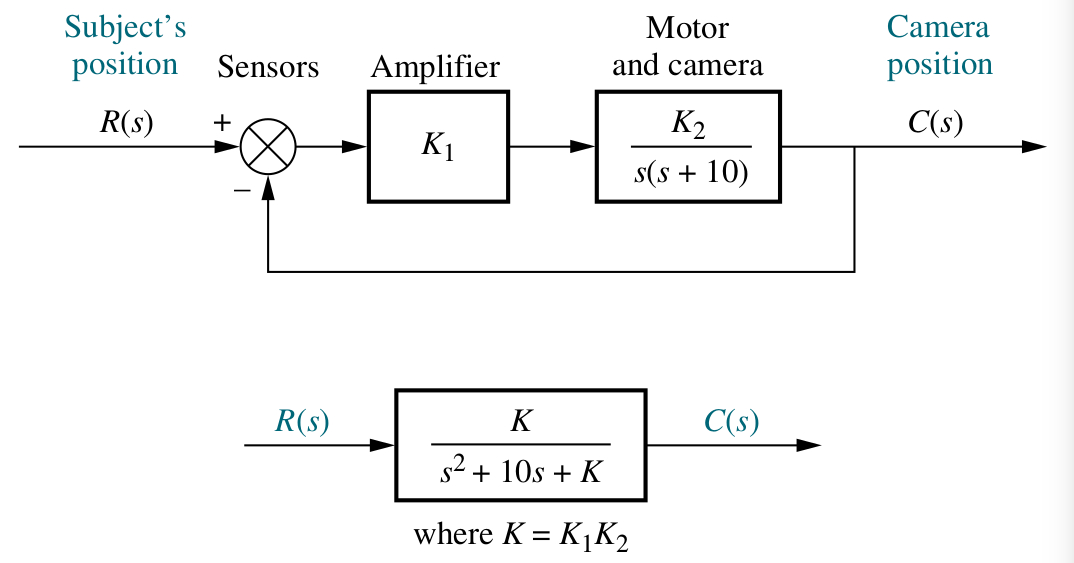
\includegraphics[width=0.68\columnwidth]{figures/Nise_Figure-8-4.jpg}
\end{figure}
\framebreak

\begin{figure}
\centering
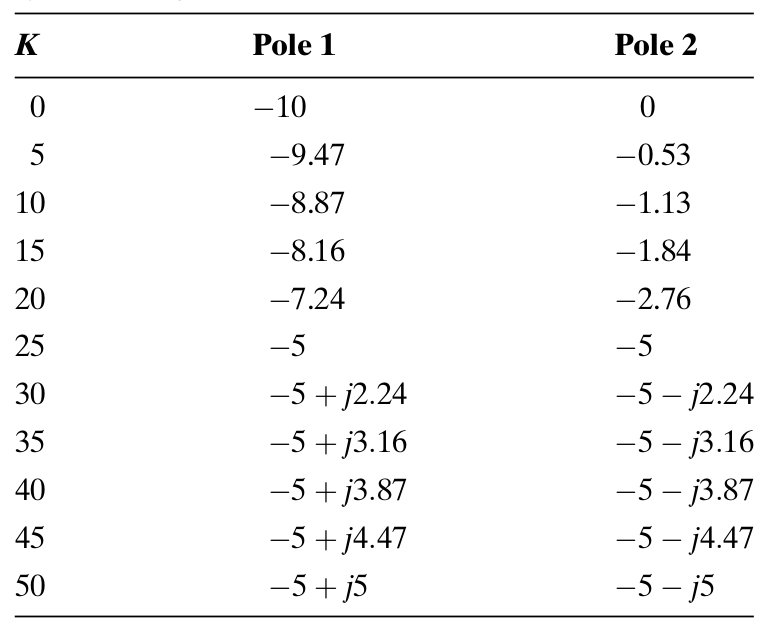
\includegraphics[width=0.56\columnwidth]{figures/Nise_Table-8-1.jpg}
\end{figure}

\end{frame}

% -----------------------------------------------------------------
\begin{frame}[allowframebreaks]
\frametitle{\insertsection}

The root locus concerns the design of closed-loop control systems with the following architecture: 
\begin{figure}
\centering
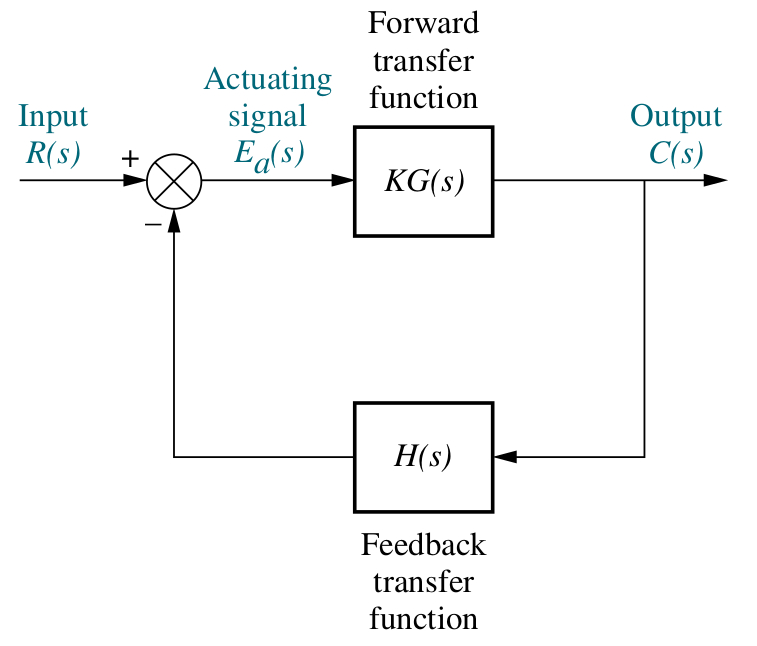
\includegraphics[width=0.5\columnwidth]{figures/Nise_Figure-8-1.jpg}
\end{figure}
\framebreak

Definitions: 
\begin{itemize}
\item Loop gain: $K$
\item Open-loop transfer function: $G(s) \, H(s)$
\end{itemize}
\fullskip

Objective: 
\begin{itemize}
\item Sketch the roots of the closed-loop transfer function as the loop gain $K$ \linebreak ranges from near zero (\ie $K \rightarrow 0^+$) to infinity (\ie $K \rightarrow +\infty$). 
\end{itemize}

\end{frame}

% =================================================================
\subsection{Sketching Rules}

% -----------------------------------------------------------------
\begin{frame}[allowframebreaks]
\frametitle{\insertsection}

Root locus sketching rules:
\begin{itemize}
\item The root locus is symmetric about the real axis. 
\item The number of branches, \ie pole trayectories, equals the number of poles \linebreak of the open-loop transfer function. 
\item Each branch begins at an open-loop pole and ends either: 
\begin{itemize}
\item At an open-loop zero. 
\item At infinity along an asymptote. 
\end{itemize}
\item Along the real line, root locus branches can be found to the left of any \linebreak odd number of real open-loop poles or open-loop zeros. 
\framebreak

\item If the root locus has asymptotes, then the number of asymptotes is: 
\[
\text{ ( number of open-loop poles ) } -  
\text{ ( number of open-loop zeros ) }
\]
\item If the root locus has asymptotes, then the centroid of the asymptotes is located along the real axis at the point: 
\[
\sigma_a \; = \; 
\frac{ \sum \text{(open-loop pole locations)} - \sum \text{(open-loop zero locations)} }{ \text{number of asymptotes} }
\]
\item If the root locus has asymptotes, then their angles in radians are: 
\[
\theta_a \; = \; 
\frac{ ( 2k + 1 ) \, \pi }{ \text{number of asymptotes} }
\qquad
\text{for } k \, = \, 0, \, \pm 1, \, \pm 2, \, \dots
\]
\end{itemize}

\end{frame}

\end{document}
